% ======================================================================
% Scientific report for the compass-needle lattice project -- Report V60
% Restructured October 2026 after docs/AUDITORIA_RELATORIO.md:
% methods and results; software usage lives in USER_GUIDE.md.
% Compile from docs/:  pdflatex project_report.tex  (twice, for the TOC)
% Figures: ../figs/*.png (geometries) and figs/*.pdf (results, generated by
% fase2_analysis.py and fase2_qs_analysis.py).
% ======================================================================
\documentclass[11pt,a4paper]{article}

\usepackage[utf8]{inputenc}
\usepackage[T1]{fontenc}
\usepackage[english]{babel}
\usepackage{geometry}
\geometry{margin=2.35cm}
\usepackage{booktabs}
\usepackage{longtable}
\usepackage{array}
\usepackage{amsmath}
\usepackage{amssymb}
\usepackage{siunitx}
\usepackage{xcolor}
\usepackage{hyperref}
\usepackage{enumitem}
\usepackage{listings}
\usepackage{caption}
\usepackage{graphicx}
\usepackage{tikz}
\usetikzlibrary{arrows.meta,calc,positioning}
\hypersetup{colorlinks=true, linkcolor=blue!50!black, urlcolor=blue!50!black,
            citecolor=blue!50!black}
\captionsetup{font=small, labelfont=bf}

\newcommand{\code}[1]{\texttt{#1}}
\newcommand{\vect}[1]{\boldsymbol{#1}}

\lstdefinestyle{bashstyle}{
  basicstyle=\ttfamily\small,
  breaklines=true,
  frame=single,
  columns=fullflexible,
  backgroundcolor=\color{gray!6},
  rulecolor=\color{gray!40}
}
\lstdefinestyle{csvstyle}{
  basicstyle=\ttfamily\scriptsize,
  breaklines=true,
  frame=single,
  columns=fullflexible,
  backgroundcolor=\color{gray!6},
  rulecolor=\color{gray!40}
}

% Automatic time calculation macros
\newcount\hh
\newcount\mm
\hh=\time
\divide\hh by 60
\mm=\hh
\multiply\mm by 60
\mm=-\mm
\advance\mm by \time
\newcommand{\hhmm}{\ifnum\hh<10 0\fi\number\hh:\ifnum\mm<10 0\fi\number\mm}


\providecommand{\todo}[1]{\textcolor{red!70!black}{\textbf{[#1]}}}

\title{\textbf{Inertia, damping and sweep rate in two-dimensional\\
dipolar compass-needle arrays}\\[1ex]
\large Scientific report V60: model, numerical methods, validation and results}
\author{J.~P.~Sinnecker}
\date{\today, \hhmm\\[0.5ex]
\small Code: \code{compass.py} 2.1.0 with the October 2026 Phase-1 fixes and the quasi-static protocol\\
(git branch \code{fase2/dynamic-hysteresis}); usage: \code{USER\_GUIDE.md}}

\begin{document}
\maketitle

\begin{abstract}
\noindent
We study two-dimensional arrays of macroscopic compass needles: rigid planar rotors carrying point dipoles on fixed pivots, coupled by the full long-range dipolar interaction and obeying Newton's equation for rotation with viscous damping. The question is whether inertia and damping, summarized by an intrinsic quality factor $Q_0$, change collective reversal (hysteresis, avalanches, memory) in square, triangular and honeycomb arrays.
An audit of the earlier simulations showed that their apparent $Q$ dependence was dominated by numerical and protocol artefacts. A dipolar cutoff biased the interior field by 15--17\,\%. The time step was under-resolved (1.4--1.8\,\% energy error at zero damping). $Q$ depended on the field amplitude. Above all, the field sweep rate was uncontrolled: the loop area scales as $\sim$(rate)$^{0.6}$.
After correcting these issues, and with every correction covered by automated physics tests, we report two campaigns. (i) 690 hysteresis cycles at a controlled dimensionless sweep rate $r$ ($6\times6$ to $64\times64$ needles) show that for $Q_0\lesssim1$ the loops collapse when the rate is measured in units of the viscous relaxation time, and that at finite rate inertia narrows the loop by 20--50\,\%. (ii) 120 loops computed with a new event-driven quasi-static protocol show that in the limit $r\to0$ the loop is set almost entirely by the energy landscape. $Q_0=1$ coincides with the gradient flow, and loops do not depend on the initial state. Inertia acts through discrete path-selection events: rare, but changing the loop area by up to 15--43\,\% at specific geometries and sizes.
Inertia therefore matters mainly for \emph{dynamic} hysteresis and for the selection of reversal paths, not as a smooth modification of the quasi-static loop.
\end{abstract}

\tableofcontents
\newpage

% ======================================================================
\section{Introduction}
\label{sec:intro}
% ======================================================================

Arrays of interacting magnetic dipoles are a classic model system for collective magnetism: frustration, domains, hysteresis and avalanche-like reversal arise from the long-range, anisotropic dipolar coupling alone. Macroscopic realizations with compass needles have been used to study dipolar ordering and thermodynamics~\cite{olive1998} and the dependence of magnetization processes on the number and arrangement of needles~\cite{novak2004}. Nanoscale realizations, artificial spin ice (ASI), have made frustration and its dynamics a large field~\cite{nisoli2013,skjaervoe2020}, including clocked and field-protocol-controlled dynamics~\cite{jensen2024}, reversal via effective magnetic charges~\cite{mellado2010}, relaxation pathways~\cite{menniti2025} and memory for computation~\cite{taniguchi2025}.

The present system differs from ASI in a fundamental way. Nanoislands follow gyromagnetic (Landau--Lifshitz--Gilbert) dynamics and switch over shape-anisotropy barriers. A compass needle is a mechanical rotor with true moment of inertia, viscous (and in reality dry) friction, and no intrinsic switching barrier. ASI is therefore \emph{motivation only}: no claim of equivalence is made.

\paragraph{Closest prior work and the gap.} Macroscopic arrays of rotatable magnets with explicit inertia and dissipation have already been built and modelled. A planar lattice of magnetic rotors relaxes into a spin-ice phase over several time scales, and it was argued that microscopic ASI cannot capture inertial effects~\cite{mellado2012}. Chains of dipolar rotors have been used to design hysteresis, with the rotor time scale bounding the sweep rate below which the loop becomes rate-independent~\cite{concha2017}. Separately, the dependence of the loop area on sweep rate (\emph{dynamic hysteresis}) is a classic problem with scaling laws $A-A_0\propto R^{\beta}$~\cite{rao1990}. What is missing is a controlled separation, in a long-range dipolar lattice, of three things: the quasi-static loop $A_0$, its dynamic excess $A-A_0$, and the role of inertia in each of them, across geometries and sizes. That separation is the subject of this report.

\paragraph{What this report contains.} Section~\ref{sec:model} defines the model and its scales; Sec.~\ref{sec:methods} the numerical methods, including the event-driven quasi-static protocol; Sec.~\ref{sec:validation} their validation. Section~\ref{sec:res_audit} quantifies the defects found in the earlier simulations; Sec.~\ref{sec:res_dynamic} reports dynamic hysteresis at controlled rate; Sec.~\ref{sec:res_qs} the quasi-static limit and the per-step avalanches. Section~\ref{sec:discussion} discusses what is a rate effect and what is inertial; Secs.~\ref{sec:limitations} and~\ref{sec:next} list limitations and next steps. Software usage (flags, file formats, commands) is documented only in \code{USER\_GUIDE.md}.

% ======================================================================
\section{Model}
\label{sec:model}
% ======================================================================

\subsection{Needle and lattices}

Each needle is a flat diamond-shaped steel lamina with a central pivot (Fig.~\ref{fig:needle_geometry}). In the model it is reduced to a rigid planar rotor at a fixed lattice site $\vect r_i$ with one angular degree of freedom $\theta_i$ and moment $\vect m_i=m(\cos\theta_i,\sin\theta_i,0)$. The blade shape is used only to compute $m=M_s\,t\,LW/2$ and the moment of inertia $I=\tfrac1{24}m_{\rm blade}(L^2+W^2)$ (rhombus of length $L=\SI{10}{mm}$ and width $W=\SI{3}{mm}$; $M_s=\SI{1.59e6}{A/m}$, steel density \SI{7850}{kg/m^3}). The pivot spacing is \SI{13}{mm}.

\textbf{Open item: thickness.} The drawing and the small prototype use $t=\SI{0.26}{mm}$, whereas all simulations reported here use the engine default $t=\SI{0.4}{mm}$. Since $m\propto t$ and $I\propto t$, the thickness rescales $B_{\rm ref}$ and the time unit but not the dimensionless results ($Q_0$, $r$, fields in units of $B_{\rm ref}$). It must nevertheless be fixed against the real needle before comparison with experiment.

\begin{figure}[htbp]
\centering
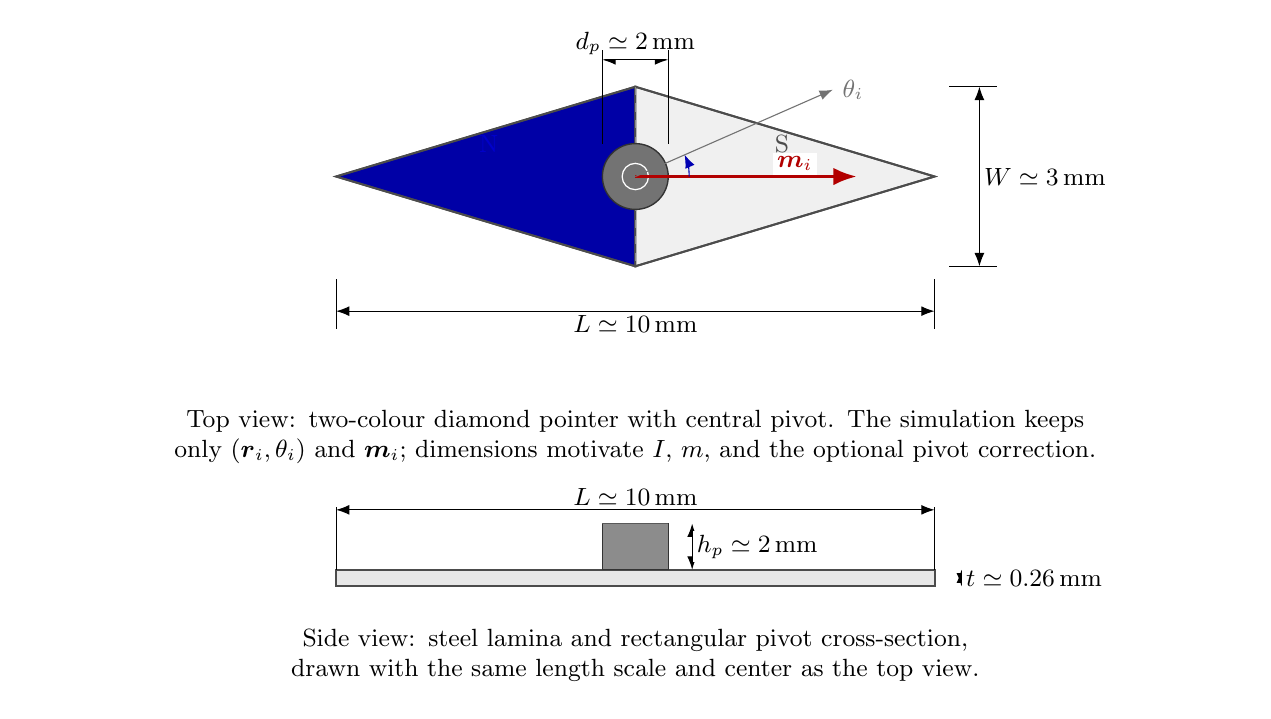
\begin{tikzpicture}[
    >=Latex,
    scale=0.76,
    every node/.style={font=\small},
    dim/.style={Latex-Latex,thin},
    lab/.style={fill=white,inner sep=1.5pt},
    steel/.style={draw=black!70,line width=0.7pt},
    north/.style={fill=blue!65!black},
    south/.style={fill=gray!12},
    pivot/.style={fill=black!55,draw=black!80,line width=0.5pt}
]
% top-view coordinates: 10 mm by 3 mm, drawn in arbitrary units
\coordinate (Ltip) at (-5,0);
\coordinate (Rtip) at (5,0);
\coordinate (Top)  at (0,1.5);
\coordinate (Bot)  at (0,-1.5);
\coordinate (C)    at (0,0);

% two magnetic halves of the diamond needle
\path[steel,north] (Ltip) -- (Top) -- (C) -- (Bot) -- cycle;
\path[steel,south] (C) -- (Top) -- (Rtip) -- (Bot) -- cycle;
\draw[steel] (Ltip) -- (Top) -- (Rtip) -- (Bot) -- cycle;
\draw[black!45,dashed] (Top) -- (Bot);

% central pivot / bearing disk
\shade[ball color=black!50] (C) circle (0.55);
\draw[pivot] (C) circle (0.55);
\draw[white,line width=0.45pt] (C) circle (0.22);

% magnetic moment and angle
\draw[->,very thick,red!70!black] (C) -- (3.7,0) node[above,pos=0.72,lab] {$\vect m_i$};
\draw[->,blue!70!black] (C) ++(0.9,0) arc[start angle=0,end angle=24,radius=0.9];
\draw[->,black!55] (C) -- ++(3.3,1.45) node[right] {$\theta_i$};
\node[blue!80!black] at (-2.45,0.55) {N};
\node[black!70] at (2.45,0.55) {S};

% length and width dimensions
\draw[dim] (-5,-2.25) -- (5,-2.25) node[midway,below,lab] {$L\simeq\SI{10}{mm}$};
\draw[thin] (-5,-1.72) -- (-5,-2.55);
\draw[thin] (5,-1.72) -- (5,-2.55);
\draw[dim] (5.75,-1.5) -- (5.75,1.5) node[midway,right,lab] {$W\simeq\SI{3}{mm}$};
\draw[thin] (5.25,-1.5) -- (6.05,-1.5);
\draw[thin] (5.25,1.5) -- (6.05,1.5);

% pivot diameter callout
\draw[dim] (-0.55,1.95) -- (0.55,1.95) node[midway,above,lab] {$d_p\simeq\SI{2}{mm}$};
\draw[thin] (-0.55,0.55) -- (-0.55,2.12);
\draw[thin] (0.55,0.55) -- (0.55,2.12);

% compact model-reduction note, placed below the top view to avoid overlap
\node[align=center,font=\small,text width=15.2cm] at (0,-4.35)
{Top view: two-colour diamond pointer with central pivot. The simulation keeps only $(\vect r_i,\theta_i)$ and $\vect m_i$; dimensions motivate $I$, $m$, and the optional pivot correction.};

% side-view inset: same horizontal scale and center as the top view
\begin{scope}[shift={(0,-6.85)}]
  \draw[steel,fill=gray!18] (-5,0) rectangle (5,0.28);
  \draw[thin] (-5,0.28) -- (-5,1.32);
  \draw[thin] (5,0.28) -- (5,1.32);
  \draw[dim] (-5,1.28) -- (5,1.28) node[midway,above,lab] {$L\simeq\SI{10}{mm}$};
  \draw[pivot,fill=black!45] (-0.55,0.28) rectangle (0.55,1.05);
  \draw[black!65,line width=0.35pt] (-0.55,1.05) -- (0.55,1.05);
  \draw[dim] (5.45,0) -- (5.45,0.28) node[midway,right,lab] {$t\simeq\SI{0.26}{mm}$};
  \draw[dim] (0.95,0.28) -- (0.95,1.05) node[midway,right,lab] {$h_p\simeq\SI{2}{mm}$};
  \node[align=center,font=\small,text width=15.2cm] at (0,-1.15) {Side view: steel lamina and rectangular pivot cross-section, drawn with the same length scale and center as the top view.};
\end{scope}
\end{tikzpicture}
\caption{Idealized geometry of the compass needle. The dynamics keeps only the pivot position and the angle; the blade dimensions set $I$ and $m$. The drawing shows the prototype thickness $t\simeq\SI{0.26}{mm}$; the simulations reported here use $t=\SI{0.4}{mm}$ (see text).}
\label{fig:needle_geometry}
\end{figure}

Three lattices are used, with the same nearest-neighbour distance $r_{\rm nn}$ (Figs.~\ref{fig:square_geometry}--\ref{fig:honeycomb_geometry}): square (coordination 4), triangular (6, the most frustrated) and honeycomb (3). All arrays are finite with free boundaries, as in the physical object.

\begin{figure}[htbp]
\centering
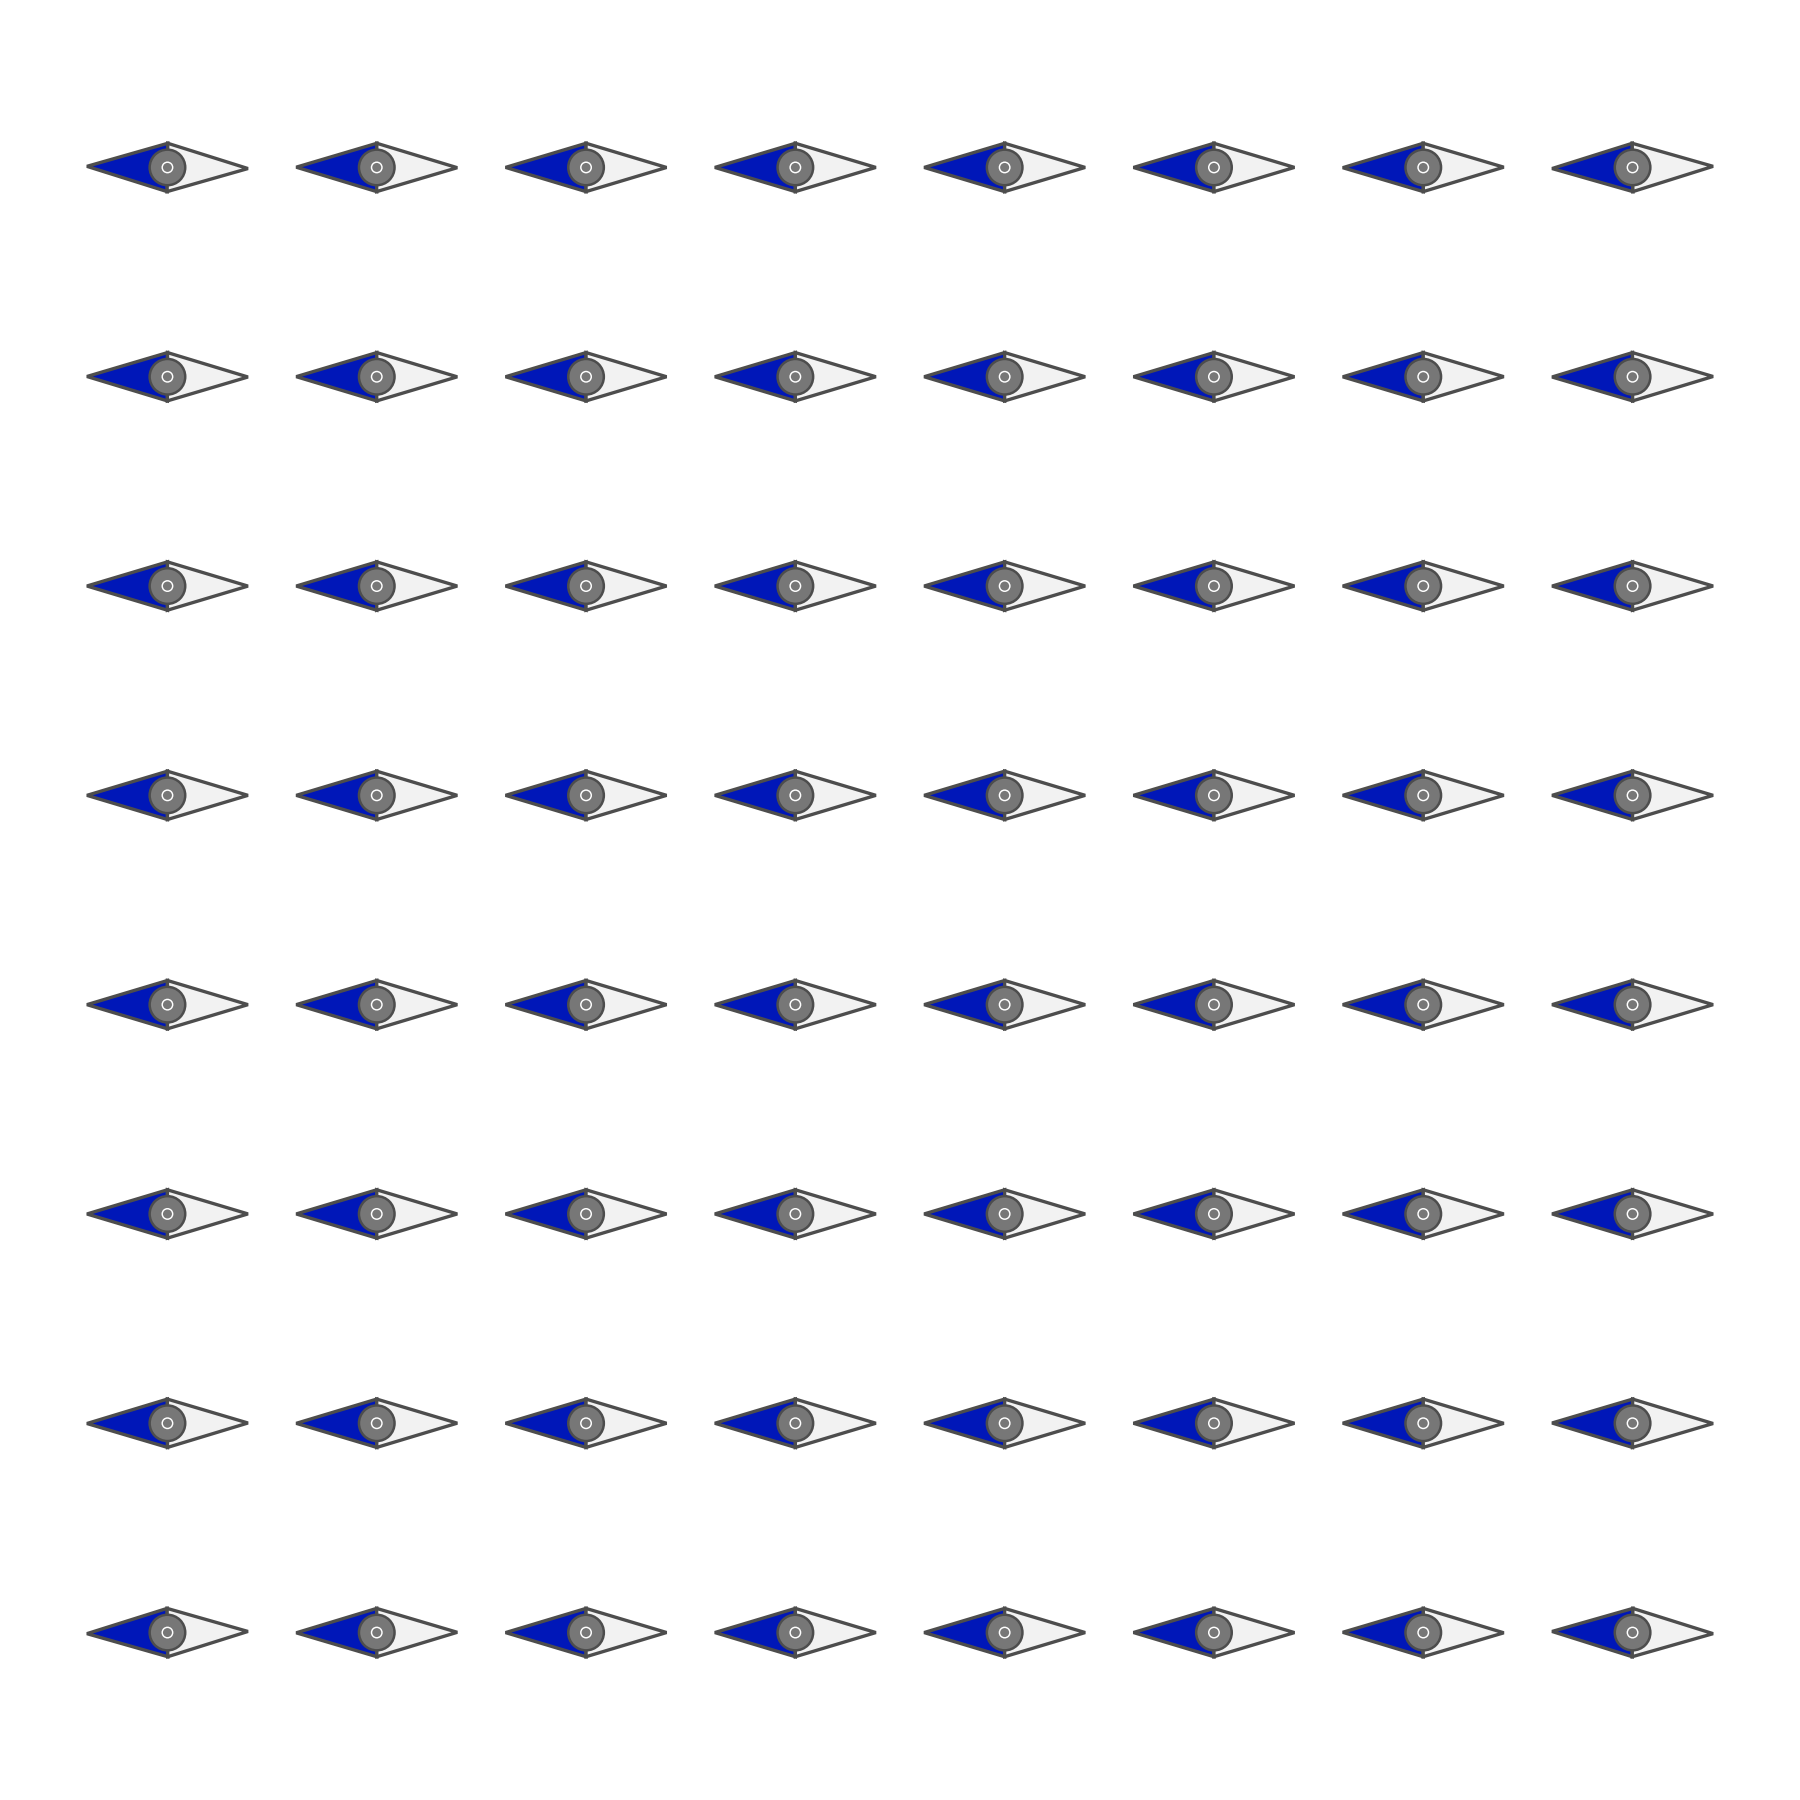
\includegraphics[width=0.62\textwidth,height=0.42\textheight,keepaspectratio]{../figs/square_default_geometry_clean_colored.png}
\caption{Square-lattice geometry used by \code{compass.py}. Pivots lie on a rectangular grid with four nearest neighbours in the bulk. This is the least frustrated of the three default geometries and provides the natural baseline for interpreting domains, hysteresis loops, and avalanche activity. Because the principal lattice directions are orthogonal, field sweeps along $x$ or $y$ have a simple relation to rows and columns of needles.}
\label{fig:square_geometry}
\end{figure}

\begin{figure}[htbp]
\centering
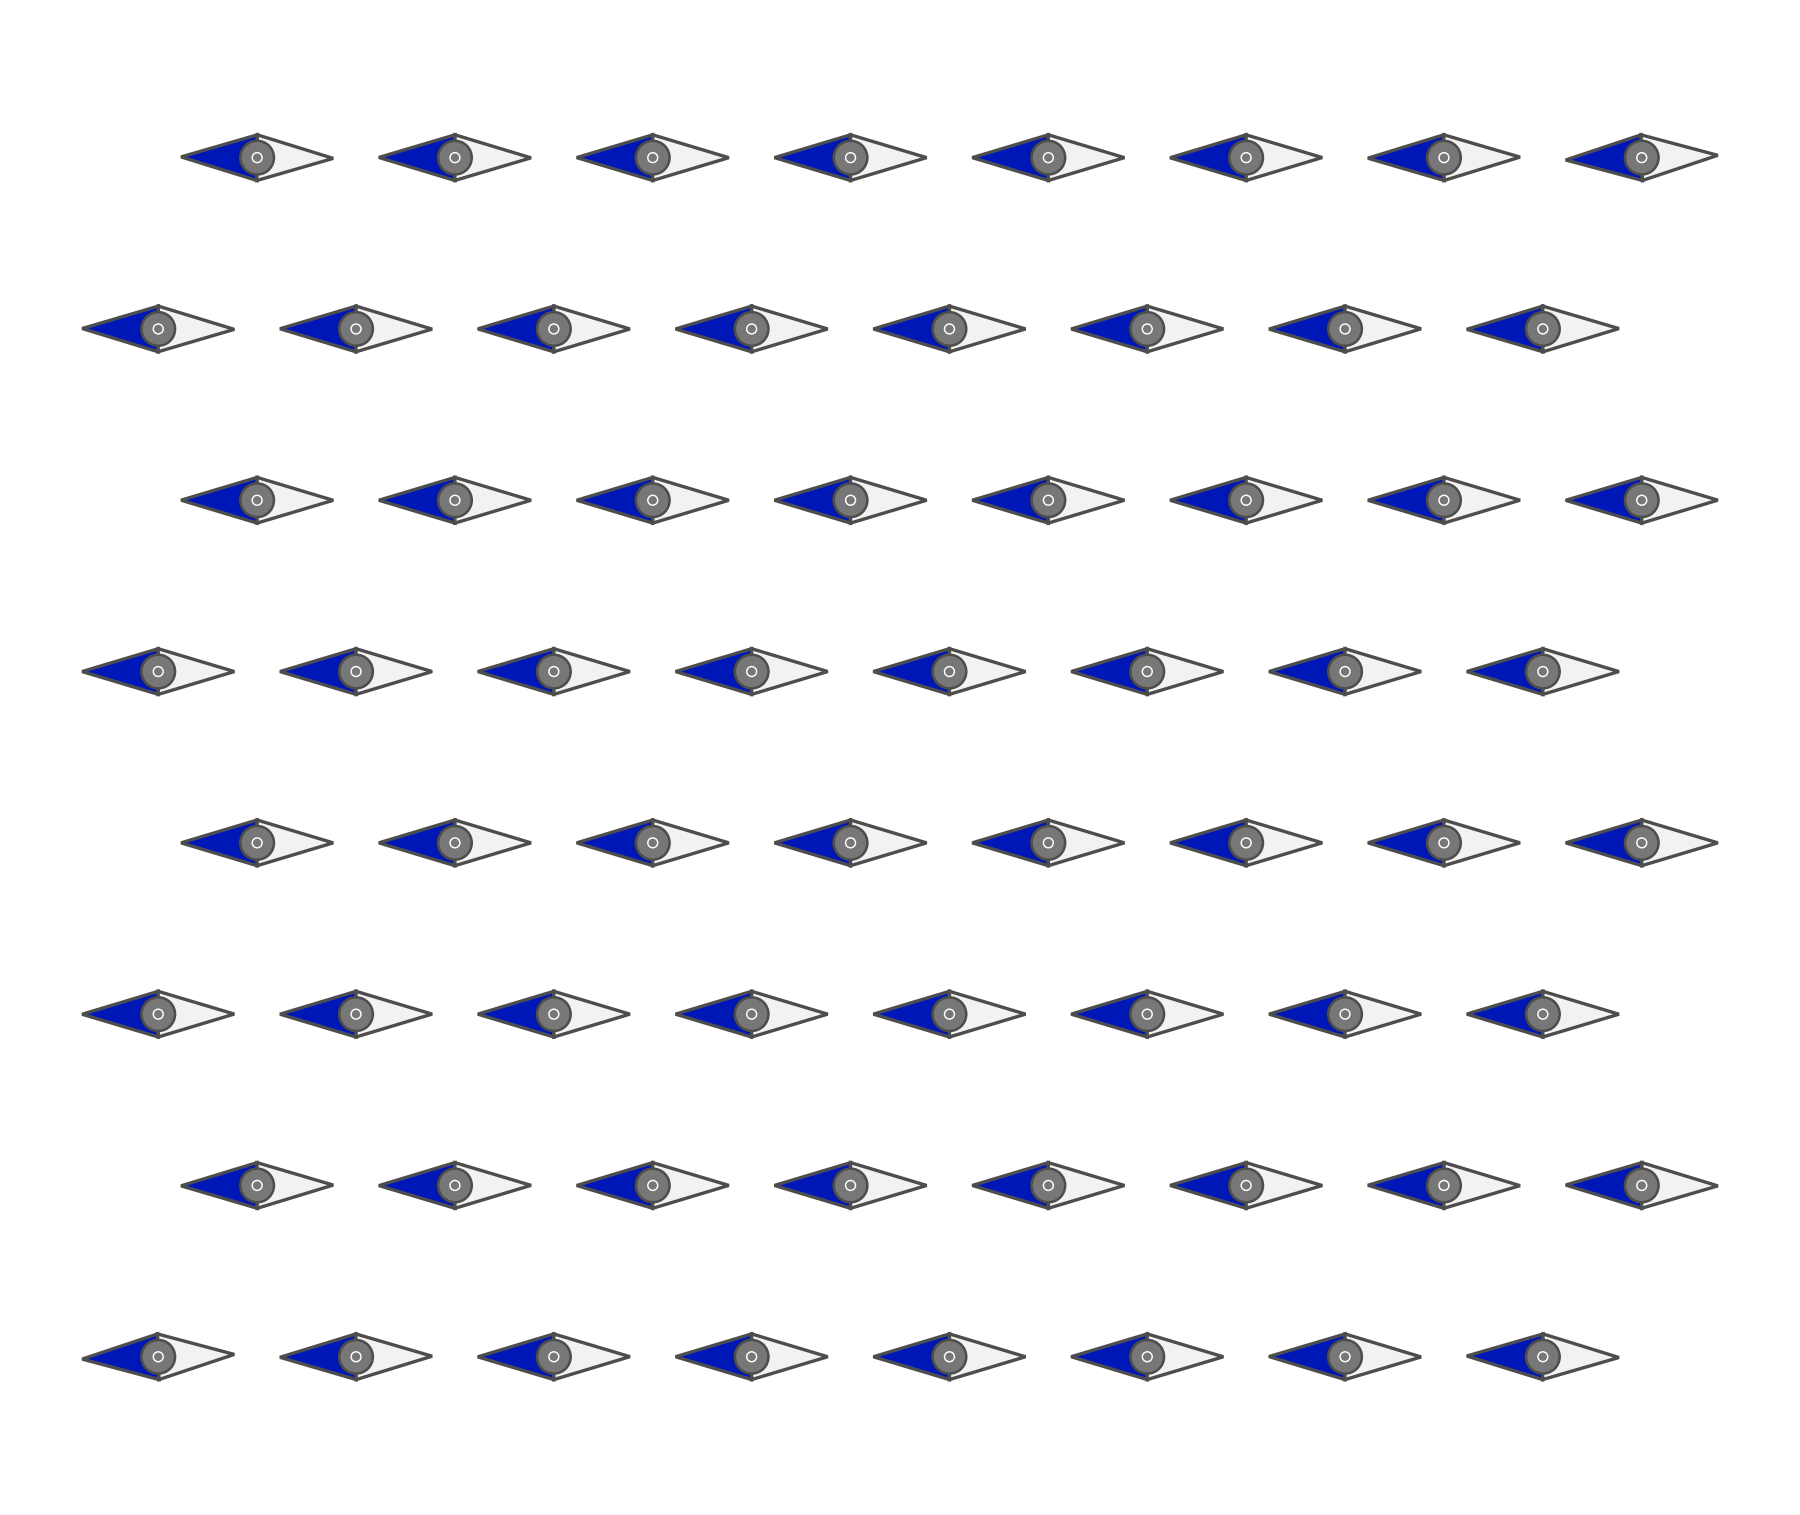
\includegraphics[width=0.62\textwidth,height=0.42\textheight,keepaspectratio]{../figs/triangular_default_geometry_clean_colored.png}
\caption{Triangular-lattice geometry. Each bulk pivot has six nearest neighbours, giving the highest local coordination among the default arrays. The equilateral triangular connectivity introduces strong geometric competition for dipolar alignment, so this geometry is expected to be especially sensitive to frustration, overshoot, and damping-controlled pathway selection. It is therefore a key test case for distinguishing purely static dipolar effects from genuinely dynamical inertial effects.}
\label{fig:triangular_geometry}
\end{figure}

\begin{figure}[htbp]
\centering
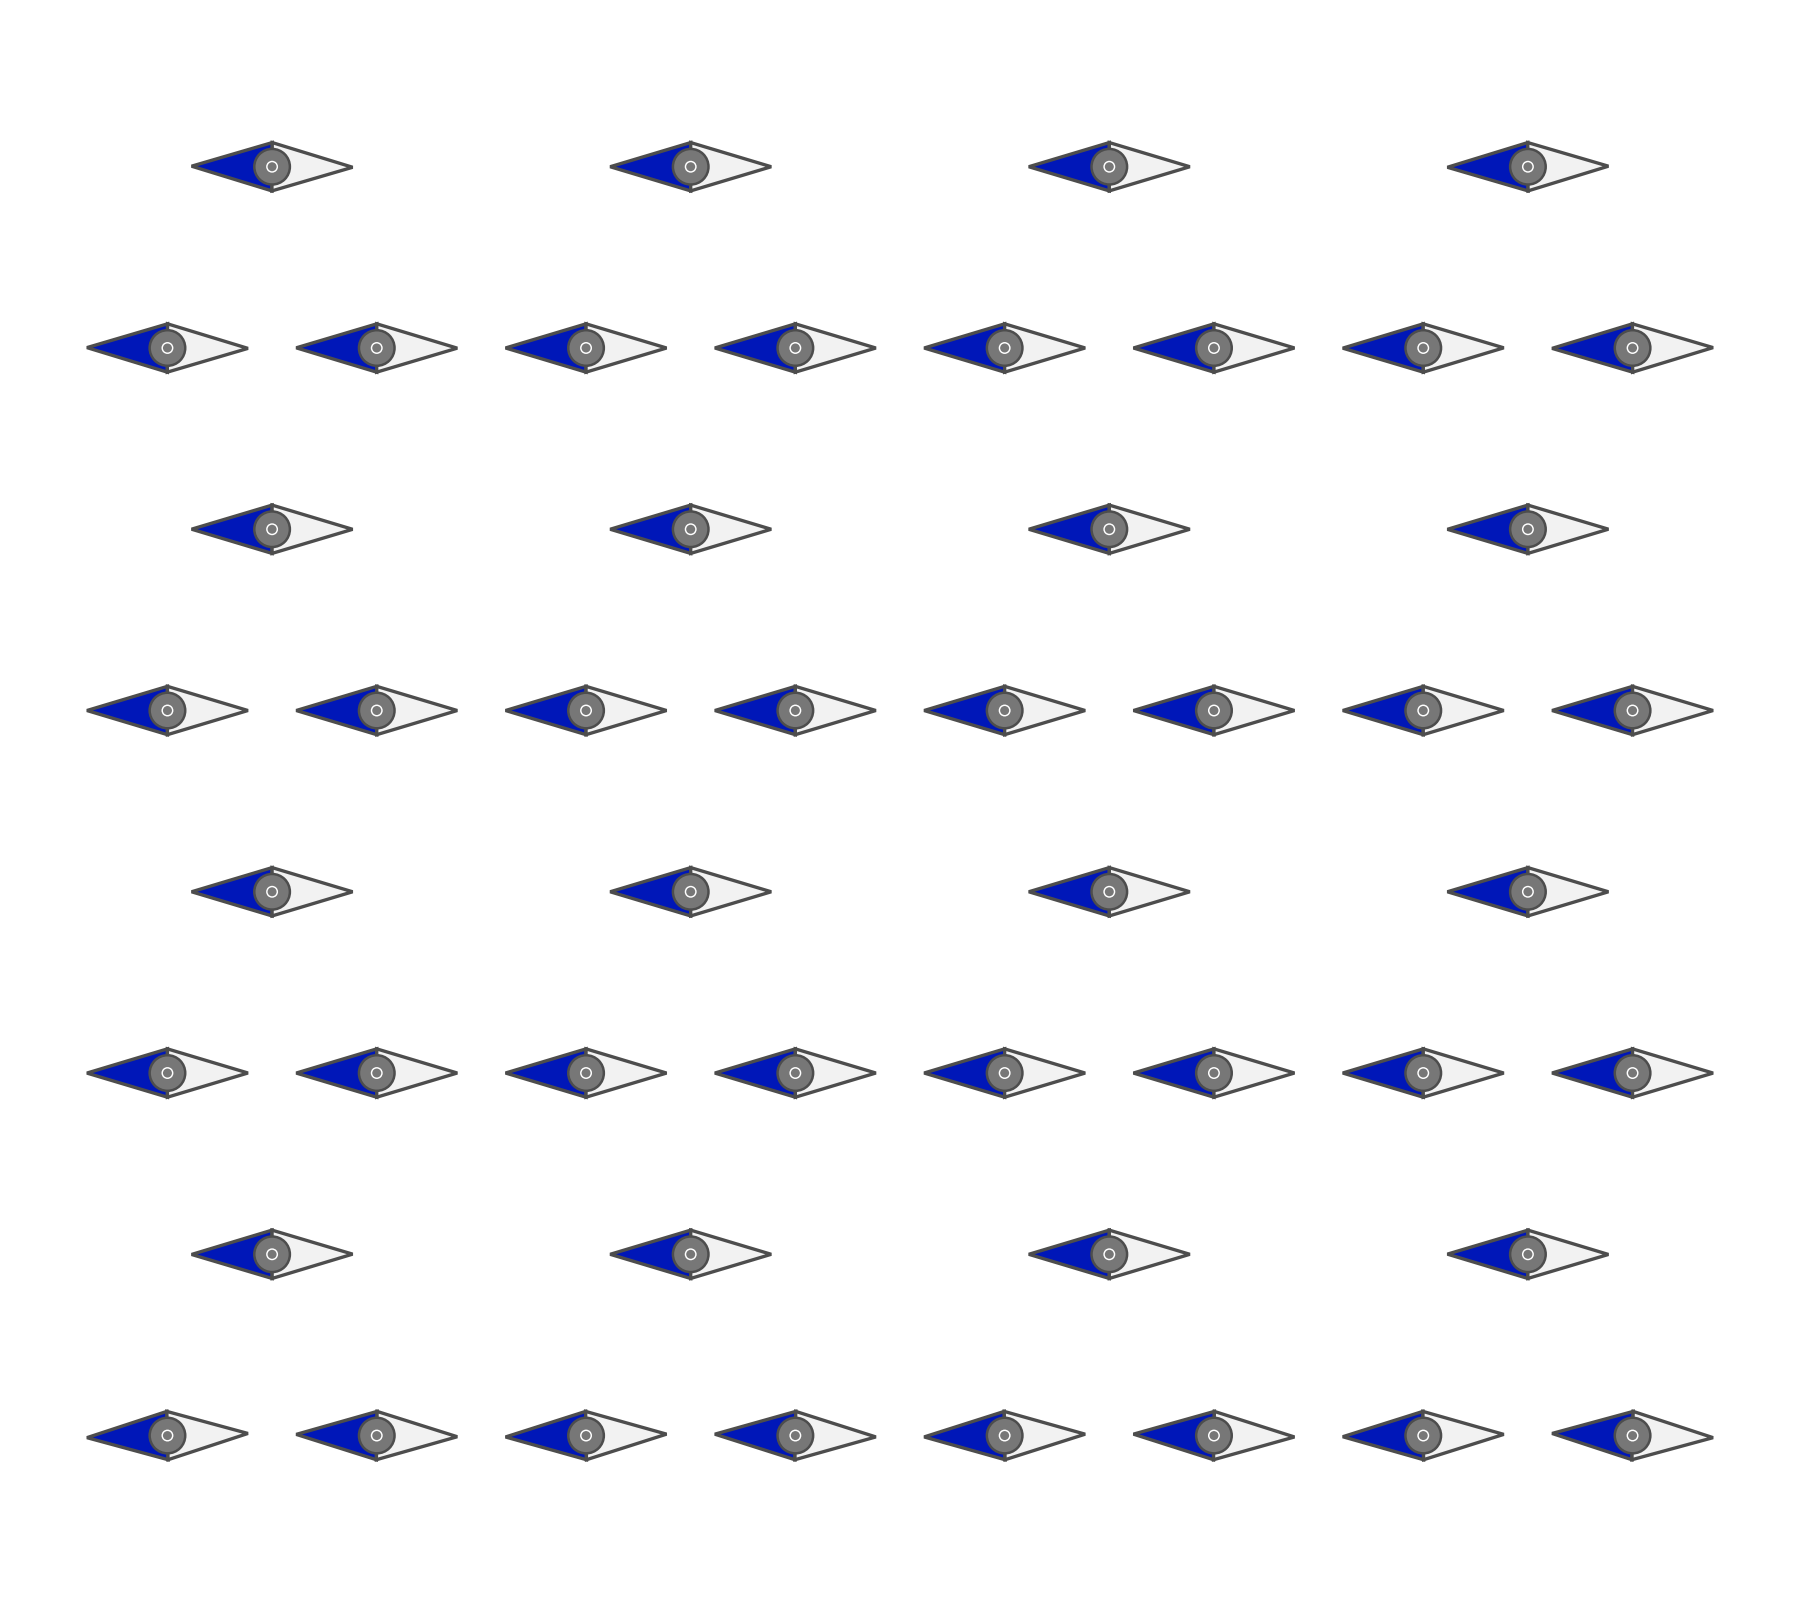
\includegraphics[width=0.62\textwidth,height=0.42\textheight,keepaspectratio]{../figs/honeycomb_default_geometry_clean_colored.png}
\caption{Honeycomb-lattice geometry. The honeycomb array can be viewed as a triangular construction with systematic removal of sites, producing hexagonal voids and three nearest neighbours per bulk pivot. This lower coordination changes both the available domain-wall paths and the local reversal constraints. It also gives a geometry closer in spirit to artificial-spin-ice networks, while retaining the continuous-angle compass-needle dynamics of the present model.}
\label{fig:honeycomb_geometry}
\end{figure}

\subsection{Interaction and dynamics}

The field at needle $i$ is the sum of the dipolar fields of all other needles and the applied field,
\begin{equation}
\vect B_i=\frac{\mu_0}{4\pi}\sum_{j\neq i}\frac{3(\vect m_j\cdot\hat{\vect r}_{ij})\hat{\vect r}_{ij}-\vect m_j}{r_{ij}^3}+\vect B_{\rm ext}(t),
\qquad \tau_i=(\vect m_i\times\vect B_i)_z ,
\end{equation}
and each needle obeys
\begin{equation}
I\ddot\theta_i=\tau_i-b\,\dot\theta_i .
\label{eq:eom}
\end{equation}
The model is deterministic ($T=0$): randomness enters only through the initial angles. The energy is $E=E_{\rm dip}+E_{\rm ext}+E_{\rm kin}$ with $E_{\rm dip}=-\tfrac12\sum_i\vect m_i\cdot\vect B_i^{\rm dip}$, $E_{\rm ext}=-\sum_i\vect m_i\cdot\vect B_{\rm ext}$ and $E_{\rm kin}=\tfrac12I\sum_i\dot\theta_i^2$.

\subsection{Scales: reference field, lattice field, quality factor and sweep rate}

\begin{itemize}[leftmargin=*]
\item $B_{\rm ref}=\frac{\mu_0}{4\pi}\frac{2m}{r_{\rm nn}^3}$ is a \emph{normalization}: the on-axis field of one neighbour. Applied fields are quoted in units of $B_{\rm ref}$ (here $B_{\max}=4B_{\rm ref}$).
\item $B_{\rm lat}$ is the intrinsic field scale of the array: the median over sites of $|\vect B_i^{\rm dip}|$ in uniform states, averaged over directions. It is $\approx2.2\,B_{\rm ref}$ for large square arrays, smaller for small arrays because of their edges.
\item The quality factor $Q_0=\omega_{\rm lat}I/b$ with $\omega_{\rm lat}=\sqrt{mB_{\rm lat}/I}$ is independent of the field protocol.
\item The relaxation time is $\tau_{\rm relax}=\max(1/\omega_{\rm lat},\,b/(mB_{\rm lat}))=\max(1,1/Q_0)/\omega_{\rm lat}$: inertial for $Q_0\ge1$, viscous for $Q_0<1$.
\item The dimensionless sweep rate is $r=(dB/dt)\,\tau_{\rm relax}/B_{\rm ref}$: the field change, in units of $B_{\rm ref}$, during one relaxation time. The quasi-static limit is $r\to0$.
\end{itemize}

% ======================================================================
\section{Numerical methods}
\label{sec:methods}
% ======================================================================

\paragraph{Dipolar sum.} The interaction is precomputed as a dense $K\times K$ tensor, and the field is a matrix--vector product. The default is the \emph{full pair sum} over the finite array: a cutoff saves no time with a dense tensor and only biases the field (Sec.~\ref{sec:res_audit}).

\paragraph{Integrator.} Equation~\eqref{eq:eom} is integrated with velocity Verlet, treating the damping implicitly:
\begin{equation}
\omega_i^{n+1}=\frac{\omega_i^{n}\left(1-\frac{b\Delta t}{2I}\right)+\frac{\Delta t}{2I}\left(\tau_i^{n}+\tau_i^{n+1}\right)}{1+\frac{b\Delta t}{2I}} .
\end{equation}
The scheme is symplectic at $b=0$ and stable for any $b$.

\paragraph{Time step.} $\Delta t=f_{\rm dt}\,T_{\rm loc}$ with $T_{\rm loc}=2\pi/\sqrt{mB_{\rm loc}/I}$. Here $B_{\rm loc}=m\max_i\max_{\hat u}\sum_j|A_{ij}\hat u|+\max_t|B_{\rm ext}|$ bounds the field any needle can feel in \emph{any} configuration ($\approx6$--$8\,B_{\rm ref}$). Then $\omega_{\rm loc}\Delta t\le2\pi f_{\rm dt}=0.157$ for the default $f_{\rm dt}=0.025$.

\paragraph{Energy ledger.} The cumulative field work $W=-\sum_i\int\vect m_i\cdot d\vect B_{\rm ext}$ and dissipation $D=\int\sum_ib\,\dot\theta_i^2\,dt$ are integrated alongside (trapezoidal rule). They satisfy $\Delta E=W-D$ to $O(\Delta t^2)$, and over a closed field cycle $W$ equals the loop area. The loop area is computed from the ledger, and cross-checked against $-\oint M\,dB$ to $5\times10^{-3}$.

\paragraph{Protocols.} (a) \emph{Rate sweeps}: the five-branch loop $0\to+B_{\max}\to0\to-B_{\max}\to0\to+B_{\max}$ at a fixed dimensionless rate $r$; the area is measured on the closed cycle that starts at the first arrival at $+B_{\max}$.
(b) \emph{Event-driven quasi-static loop}: the same five branches in field steps $\Delta B=0.005\,B_{\rm ref}$. After each step the dynamics runs at fixed field until rest, defined as $\max_i|\tau_i|\le10^{-5}mB_{\rm lat}$ and $\max_i|\dot\theta_i|\le10^{-5}\omega_{\rm lat}$. One rest state is recorded per step, so the number of reversed needles and the energy dissipated in that step define an avalanche.
(c) \emph{Gradient flow}: in the quasi-static protocol the relaxation can instead follow $b\dot\theta_i=\tau_i$, the $Q_0\to0$ limit without inertia.

\paragraph{Avalanche counters.} A needle reverses when its projection on the drive axis changes sign. To ignore ringing, a Schmitt dead band of $\pm30^\circ$ around the perpendicular and a dwell time are required, so a ringing needle counts once per genuine reversal.

% ======================================================================
\section{Validation}
\label{sec:validation}
% ======================================================================

Every statement below is an automated test in \code{tests/test\_physics.py}, run before every commit.

\begin{itemize}[leftmargin=*]
\item The precomputed tensor equals the direct dipole--dipole pair sum to $10^{-12}$, and the torque equals $-\partial E/\partial\theta_i$ (finite differences).
\item At $b=0$ the energy drift scales as $\Delta t^2$ (ratio $\approx4$ when $\Delta t$ is halved). With damping, the energy never rises during free relaxation.
\item The time-step bound dominates the actual fields for random and aligned states on all geometries, and an $8B_{\rm ref}$ hysteresis run is never flagged by the stability monitor.
\item $Q_0$ is independent of the field amplitude and protocol, and $Q_0/Q_{\rm ref}=\sqrt{B_{\rm lat}/B_{\rm ref}}$.
\item The ledger balance holds to $O(\Delta t^2)$ (the residual ratio is $\approx4$ when $\Delta t$ is halved), and the closed-cycle field work equals the loop area.
\item The loop area converges as $r\to0$ on a small array.
\item Quasi-static protocol: logged states are mechanical equilibria within the tolerances; the ledger balance includes the field jumps; and the gradient flow reproduces the low-$Q_0$ inertial loop.
\end{itemize}

\paragraph{Tolerance of the quasi-static protocol.} The rest criterion matters. On a $6\times6$ square array at $Q_0=0.3$, a loose tolerance ($10^{-3}$, $\Delta B=0.02B_{\rm ref}$) gives $a_0=0.710$, because relaxation stops early near instabilities, where the dynamics slows down critically. The validated settings ($10^{-5}$, $\Delta B=0.005B_{\rm ref}$) give $a_0=0.461$ for inertial dynamics and $0.4606$ for the gradient flow. The slowest rate sweep ($r=3\times10^{-4}$) gives $0.473$. Over the 120 quasi-static loops, 373 of the 480\,000 field steps (0.08\,\%) reached the relaxation-time cap before the tolerance. All of them occurred in gradient-flow or $Q_0=1$ runs on large arrays, where very soft modes relax slowly.

% ======================================================================
\section{Results I: what was wrong in the earlier simulations}
\label{sec:res_audit}
% ======================================================================

The figures of the July 2026 campaign (loop area and avalanche exponent versus $Q$) were affected by four defects, quantified on the corrected code:
\begin{enumerate}[leftmargin=*]
\item \textbf{Cutoff.} A cutoff of $3.5\,r_{\rm nn}$ underestimated the interior field of a uniformly magnetized array by 15\,\% ($20\times20$) to 17\,\% ($36\times36$), and removed edge and shape fields entirely.
\item \textbf{Time step.} Setting $\Delta t$ from the single-neighbour field left $\omega_{\rm loc}\Delta t\approx0.5$. The energy error at $b=0$ was 1.8\,\% over \SI{2}{s} of a $12\times12$ array, against 0.14\,\% with the corrected step.
\item \textbf{Quality factor.} $Q$ was built from $\max(B_{\rm ref},B_{\rm ext})$, so the same damping gave a $\sqrt8\approx2.8$ times larger $Q$ in an $8B_{\rm ref}$ loop than in a static run. The campaign script used yet another convention.
\item \textbf{Sweep rate.} With $t_{\rm sim}$ fixed, the rate was uncontrolled. On a $12\times12$ array the loop area fell roughly as (rate)$^{0.6}$ at every $Q$ and never reached a quasi-static value. The old area-versus-$Q$ curve had the shape of a viscous (Debye-like) lag, not of collective physics.
\end{enumerate}
The avalanche exponents of the earlier analysis rested on tails of 30--40 events and are not retained.

% ======================================================================
\section{Results II: dynamic hysteresis at controlled sweep rate}
\label{sec:res_dynamic}
% ======================================================================

\paragraph{Campaign.} 600 cycles cover three geometries, $N=6,10,16,24,32$, $Q_0=0.1,0.3,1,3,10$ and $r=10^{-1}$ to $10^{-3}$ (down to $3\times10^{-4}$ for $N\le16$), plus seed checks. A GPU extension adds 90 cycles at $N=48,64$ ($Q_0=0.3,1,3$; $r\ge10^{-3}$). Damping was set per geometry and size so that $Q_0$ is exact. All 690 runs passed quality control: balance residual $\le1.2\times10^{-3}$, no stability flags, and $M\ge0.995$ at $B_{\max}$.

\begin{figure}[htbp]
\centering
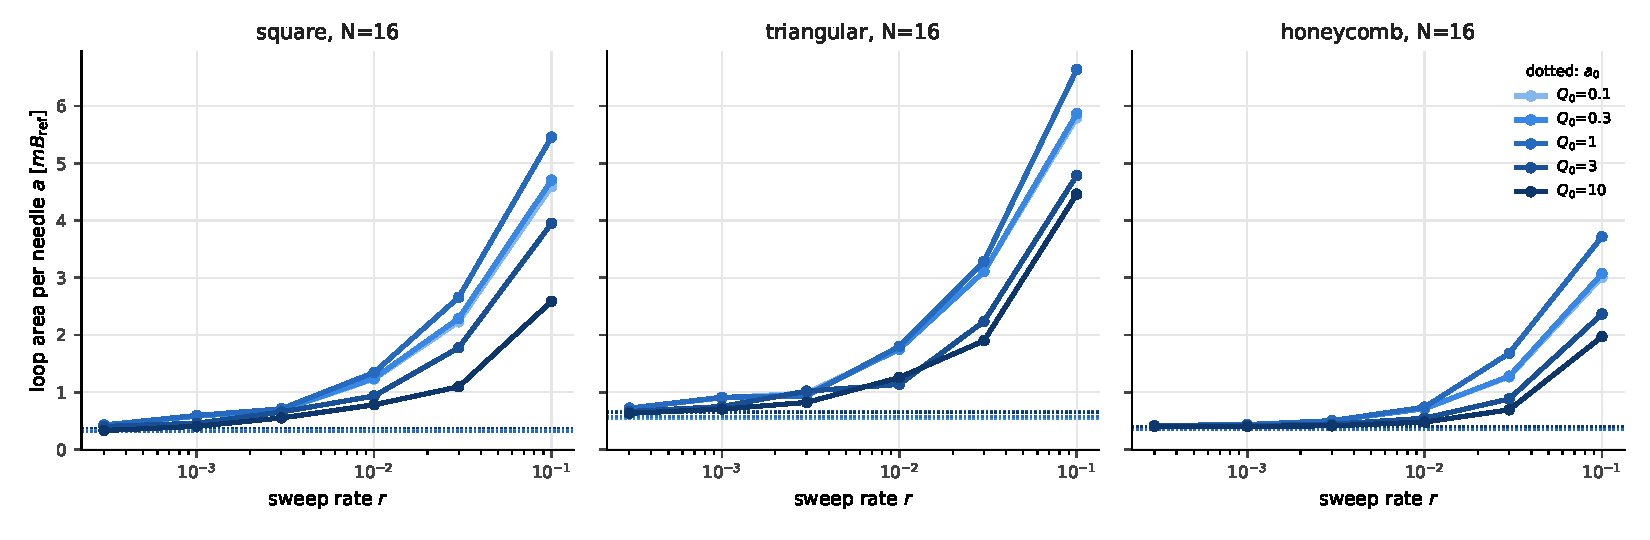
\includegraphics[width=\textwidth]{figs/fig1_area_vs_rate.pdf}
\caption{Loop area per needle $a$ (units of $mB_{\rm ref}$) versus dimensionless sweep rate $r$, $N=16$. The curves for $Q_0=0.1$, $0.3$ (and largely $1$) coincide: with $r$ measured in units of the viscous relaxation time, overdamped dynamics is a pure rescaling of time. Underdamped arrays ($Q_0=3,10$) have narrower loops at the same $r$. Dotted lines: fitted $a_0$, unreliable for the larger arrays (see text).}
\label{fig:area_rate}
\end{figure}

\paragraph{Overdamped collapse.} For $Q_0=0.1$ and $0.3$ the areas differ by at most 2.4\,\% over all geometries, sizes and rates (Fig.~\ref{fig:area_rate}). In the overdamped limit Eq.~\eqref{eq:eom} reduces to $b\dot\theta=\tau$, and $b$ only rescales time. This is a control result: any apparent $Q$ dependence for $Q\lesssim1$ at fixed $t_{\rm sim}$ is a rate effect.

\paragraph{Inertial narrowing at finite rate.} At the same $r$, raising $Q_0$ from 0.1 to 10 reduces the area by 22--44\,\% at $r=10^{-1}$ and by 28--54\,\% at $r=10^{-2}$, depending on geometry and size. Underdamped loops show ringing and discrete jumps (Fig.~\ref{fig:loops}).

\begin{figure}[htbp]
\centering
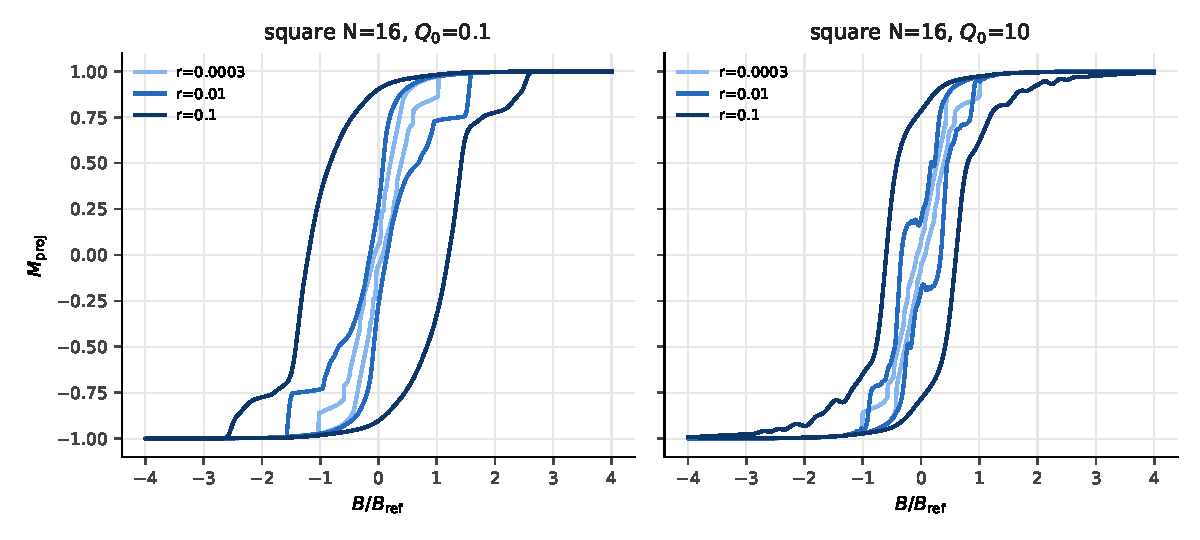
\includegraphics[width=0.85\textwidth]{figs/fig4_loops.pdf}
\caption{Hysteresis loops $M_{\rm proj}(B)$ of a $16\times16$ square array at three sweep rates, overdamped ($Q_0=0.1$, left) and underdamped ($Q_0=10$, right). Faster sweeps widen the loop; underdamped loops show ringing and discrete avalanche jumps.}
\label{fig:loops}
\end{figure}

\paragraph{The quasi-static limit is out of reach by sweeping.} For $N\ge24$ the area still changes by 40--98\,\% between $r=3\times10^{-3}$ and $10^{-3}$, and extrapolations $a(r)=a_0+c\,r^\beta$ are not reliable ($a_0$ hits zero). Reaching $r\sim10^{-5}$ by sweeping is prohibitive, since the cost grows as $1/r$, and faster still for $Q_0<1$. This motivated the quasi-static protocol of Sec.~\ref{sec:res_qs}.

\paragraph{Size dependence at fixed rate.} At $r=10^{-3}$ the area levels off for $N\ge32$. For $Q_0=0.3$: square $0.265\to0.238\to0.235$ for $N=32,48,64$; honeycomb $\approx0.42$; triangular $0.73$--$0.69$. Below $N\approx24$ the dependence is non-monotonic, reflecting edges and, for the triangular lattice, the shape of the cut.

\paragraph{Seed sensitivity in sweeps.} With uniform damping the saturated state erases the initial state in most conditions. In underdamped honeycomb arrays, however, the area varied by up to 27\,\% between seeds. Section~\ref{sec:res_qs} shows that this is a dynamic effect.

% ======================================================================
\section{Results III: the quasi-static limit and per-step avalanches}
\label{sec:res_qs}
% ======================================================================

\paragraph{Campaign.} 120 quasi-static loops cover three geometries, $N=6$--$32$, four relaxation dynamics (gradient flow, $Q_0=1,3,10$) and two seeds, with 4000 field steps each. The ledger residual was $\le8.5\times10^{-3}$ (largest for the gradient flow, whose Euler step carries a small kinetic-energy bookkeeping term).

\begin{figure}[htbp]
\centering
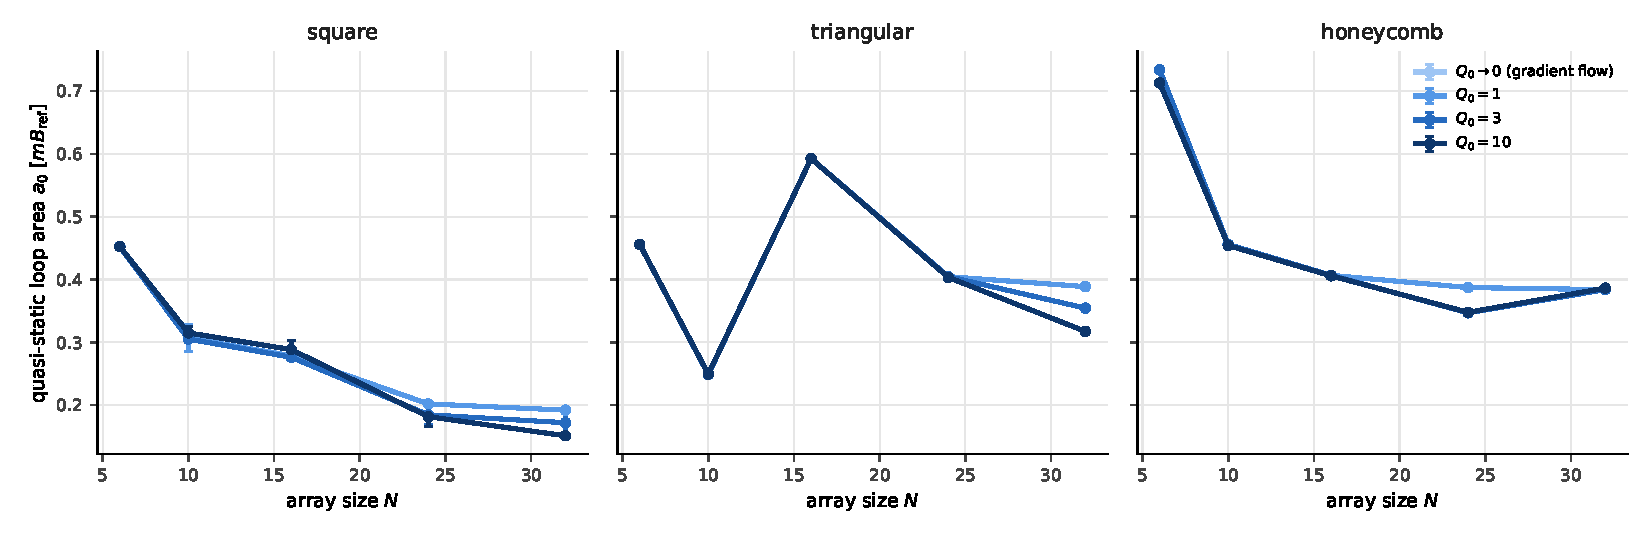
\includegraphics[width=\textwidth]{figs/figQS1_a0_vs_N.pdf}
\caption{Quasi-static loop area $a_0$ versus array size for the four relaxation dynamics (bars: range over two seeds, mostly smaller than the markers). The curves for the gradient flow and $Q_0=1$ coincide almost everywhere; departures at $Q_0=3,10$ occur at isolated geometry/size combinations.}
\label{fig:qs_a0}
\end{figure}

\paragraph{No memory of the initial state.} The two seeds give identical loops (relative spread $\le10^{-3}$) in all but four conditions, which are small honeycomb arrays ($N\le10$) at $Q_0\ge3$ (spread $\le3.2$\,\%). The large seed sensitivity seen in sweeps (Sec.~\ref{sec:res_dynamic}) is therefore a finite-rate effect.

\paragraph{$Q_0=1$ is already gradient flow.} The $Q_0=1$ loop coincides with the gradient-flow loop within 1\,\% in 13 of 15 geometry/size combinations. The exceptions are small honeycomb arrays: $6\times6$ ($+22$\,\%) and $10\times10$ ($-4$\,\%).

\begin{figure}[htbp]
\centering
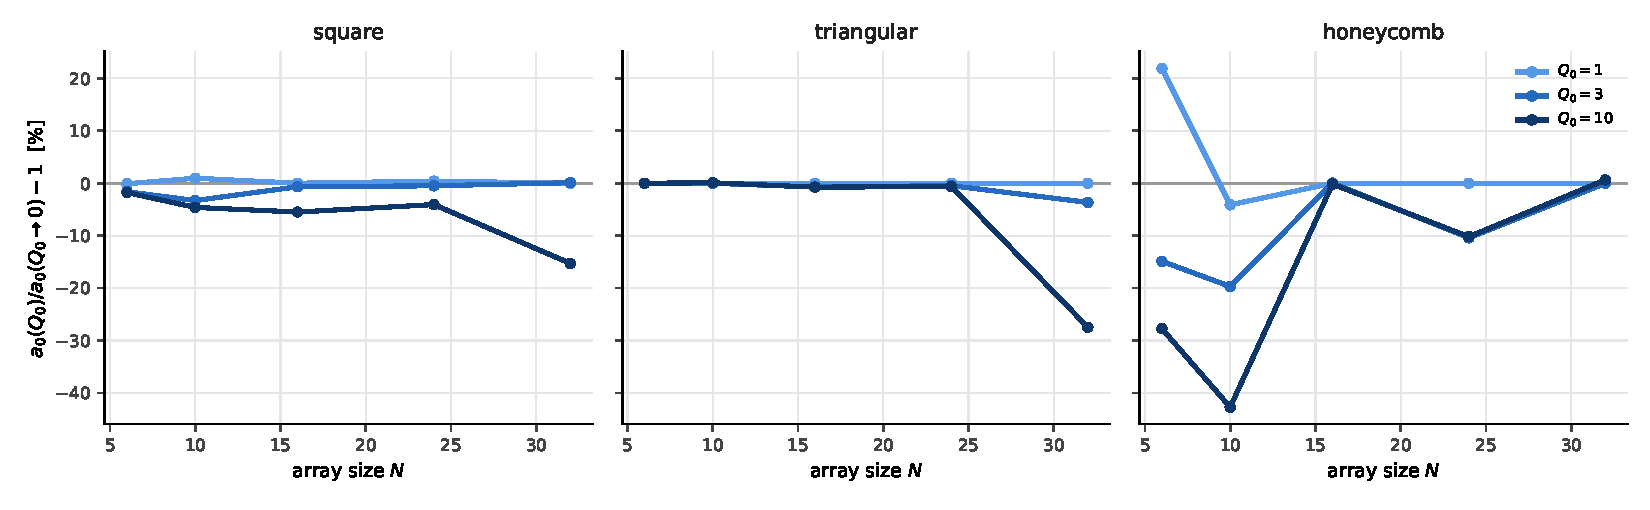
\includegraphics[width=\textwidth]{figs/figQS2_inertial_effect.pdf}
\caption{Inertial effect on the quasi-static loop: $a_0(Q_0)/a_0(Q_0\to0)-1$ versus array size.}
\label{fig:qs_effect}
\end{figure}

\paragraph{Inertia acts through discrete path selection.} In most conditions the quasi-static area changes by less than 2--5\,\% with $Q_0$ (Fig.~\ref{fig:qs_effect}). In a few it changes strongly at $Q_0=10$ (and sometimes $3$): honeycomb $10\times10$ $-43$\,\% (Q$_0=3$: $-20$\,\%), honeycomb $6\times6$ $-28$\,\%, triangular $32\times32$ $-27$\,\%, square $32\times32$ $-15$\,\%, honeycomb $24\times24$ $-10$\,\%. The effect is not monotonic in $N$ (e.g.\ honeycomb $16\times16$ and $32\times32$ show none). The coercive field and remanence change along with the area. For triangular $32\times32$ at $Q_0=10$, the remanence drops from 0.22 to 0.07.

This pattern is what one expects if, during a few large avalanches, the overshoot of the rotors carries the array into a different basin than the gradient flow would, switching the subsequent branch of the loop. Individual events, not a smooth bias, would then determine the quasi-static loop.

\begin{figure}[htbp]
\centering
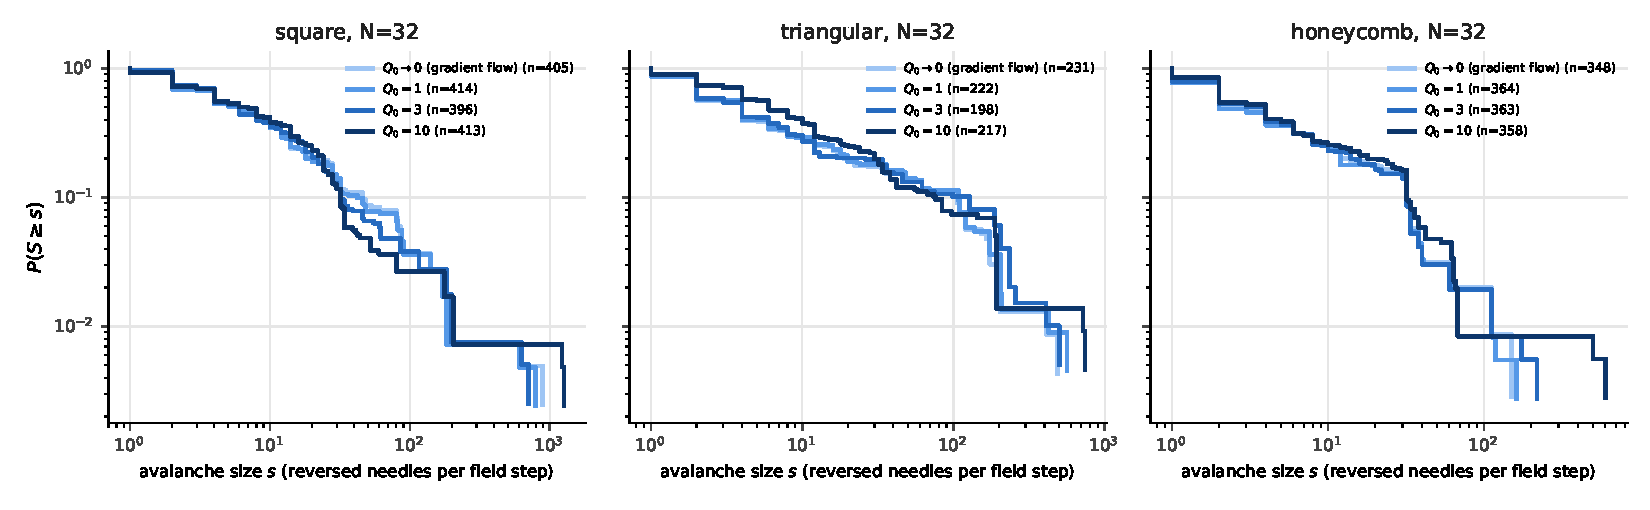
\includegraphics[width=\textwidth]{figs/figQS3_avalanche_ccdf.pdf}
\caption{Complementary cumulative distribution of the avalanche size $s$ (needles reversed per field step) for $N=32$ and the four dynamics. The distributions are similar. At $Q_0=10$ a few avalanches exceed the number of needles ($K=1024$ for the square array), i.e.\ some needles reverse more than once within one field step, a direct signature of inertial overshoot.}
\label{fig:qs_ccdf}
\end{figure}

\paragraph{Avalanches.} The per-step avalanche-size distributions are broad but strongly affected by system size (largest events of order $K$). They are similar for all dynamics (Fig.~\ref{fig:qs_ccdf}), with 200--400 events per condition (two loops) at $N=32$. At $Q_0=10$, events larger than $K$ occur. With these sizes no scaling exponent is claimed.

% ======================================================================
\section{Discussion}
\label{sec:discussion}
% ======================================================================

The picture that emerges separates cleanly into three parts:
\begin{enumerate}[leftmargin=*]
\item \textbf{Overdamped regime ($Q_0\lesssim1$): no dependence on damping.} The damping is not a parameter of the physics, only of the time scale. With $r$ measured in viscous units the loops collapse at every rate, and in the quasi-static limit $Q_0=1$ already coincides with the gradient flow.
\item \textbf{Dynamic hysteresis: large inertial effects.} At finite rate inertia reduces the loop area by tens of per cent and makes the loop depend on the initial state (honeycomb). In this sense inertia is a genuine control parameter of the \emph{dynamic} response, consistent with the rotor time scale bounding rate-independent hysteresis in dipolar chains~\cite{concha2017} and with the general phenomenology of dynamic hysteresis~\cite{rao1990}.
\item \textbf{Quasi-static loop: inertia selects paths.} In the limit $r\to0$ the energy landscape fixes the loop almost entirely. Inertia enters only through discrete events in which overshoot changes the outcome of an avalanche, which is rare but consequential, and strongly dependent on geometry and size.
\end{enumerate}
The third point connects naturally to \emph{memory}: whether a system returns to the same state after a field excursion (return-point memory) is guaranteed for overdamped ferromagnetic-like dynamics~\cite{sethna1993}, but inertial path selection is exactly the kind of mechanism that can break it. Memory formation in driven disordered matter is an active field~\cite{keim2019}, and the compass array offers a mechanical, fully characterized platform to test it. This is the proposed Phase~3.

Compared with the rotor spin-ice study of Ref.~\cite{mellado2012}, the present work adds a controlled separation of quasi-static and dynamic contributions across three geometries and sizes, a protocol-independent definition of $Q_0$, and the observation that inertia acts on the quasi-static loop through discrete path selection rather than smoothly.

% ======================================================================
\section{Limitations}
\label{sec:limitations}
% ======================================================================

\begin{itemize}[leftmargin=*]
\item \textbf{Point dipoles.} The needle length is $0.77$ of the pivot spacing, so near-field (multipolar) corrections are not small. A dumbbell (end-charge) model is needed as a robustness check.
\item \textbf{Viscous damping only.} Real pivots have dry (Coulomb) friction, which acts as a switching threshold and quenched disorder. It is absent here.
\item \textbf{$T=0$, deterministic.} There is no thermal bath. Disorder enters only through the initial state, which the quasi-static loops turn out to forget.
\item \textbf{Finite size and edges.} Arrays up to $32\times32$ (quasi-static) and $64\times64$ (sweeps), all with free boundaries. Below $N\approx24$ the size dependence is non-monotonic. The inertial events of Sec.~\ref{sec:res_qs} need a denser size scan and more seeds (or weak disorder) to establish their statistics.
\item \textbf{Quasi-static protocol.} Finite $\Delta B$ and tolerance: changing $\Delta B$ from 0.01 to $0.005B_{\rm ref}$ changes $a_0$ by 2--3\,\% on $6\times6$ arrays, and 0.08\,\% of the steps hit the relaxation cap.
\item \textbf{Thickness} not yet fixed against the real needle (dimensionless results unaffected).
\end{itemize}

% ======================================================================
\section{Next steps}
\label{sec:next}
% ======================================================================

\begin{enumerate}[leftmargin=*]
\item \textbf{Inertial path selection.} Locate the avalanches whose outcome differs between gradient flow and $Q_0=10$ (same field step, different final state), and map them in space. Then establish their frequency with more sizes and seeds, using weak damping disorder to sample realizations.
\item \textbf{Memory (Phase 3).} Nested subloops and FORC in the quasi-static protocol: does return-point memory fail with inertia, and in which geometry?
\item \textbf{Dynamic excess.} $a(r)-a_0$ with $a_0$ from the quasi-static protocol: test rate scaling and collapse across $Q_0$ and geometries.
\item \textbf{Robustness.} Dumbbell interaction, Coulomb friction as controlled disorder, sample shape.
\item \textbf{Experiment.} Measure $I$, $m$, $b$ and the static friction of real needles; compare loops at two or three rates and a memory protocol on a small array.
\end{enumerate}

\appendix
% ======================================================================
\section{Reproducibility}
\label{app:repro}
% ======================================================================

\begin{itemize}[leftmargin=*]
\item Code: \url{https://github.com/jpsinnecker/compass}, branch \code{fase2/dynamic-hysteresis}. Engine \code{compass.py}; campaigns \code{fase2\_campaign.py} (\code{--protocol sweep|qs}, sharding across machines); analysis \code{fase2\_analysis.py} and \code{fase2\_qs\_analysis.py}; tests \code{tests/}.
\item Runs: Mac (Apple M2 Max, CPU) and a Linux workstation (Intel i9-9900K CPU, NVIDIA RTX~3090 GPU for $N\ge48$). The job lists of each shard were checked to be identical on both machines.
\item Data (outside git): \code{\textasciitilde/compass\_runs/fase2*}. Each run directory has a CSV time series, JSON metadata (configuration, derived scales, energy ledger, quality-control fields) and initial/final state files.
\item Commands, flags and file formats: \code{USER\_GUIDE.md} (PDF: \code{docs/USER\_GUIDE.pdf}).
\end{itemize}

% ======================================================================
\section{Condensed history}
\label{app:history}
% ======================================================================

June--July 2026: visual simulator, geometries, field protocols, precomputed tensor (V40), FORC and demagnetization (V67--V79), research branch with metadata and observables (V2.0.2), ringing-proof avalanche counters and stability monitor (V2.1). Reports V51--V53.
October 2026: physics audit; full pair sum, time step from a local-field bound, intrinsic $Q_0$, energy ledger, dimensionless sweep rate (Phase 1, with physics tests); dynamic-hysteresis campaign and event-driven quasi-static protocol (Phase 2). Full detail: git history and \code{docs/AUDIT\_PHYSICS\_ROADMAP.md}.

% ======================================================================
\begin{thebibliography}{99}

\bibitem{olive1998}
E.~Olive and P.~Molho, \emph{Thermodynamic study of a lattice of compass needles in dipolar interaction}, Phys.\ Rev.\ B \textbf{58}, 9238 (1998).

\bibitem{novak2004}
R.~L.~Novak and J.~P.~Sinnecker, \emph{Macroscopic system for studies of magnetic dipolar interaction in small particles}, J.\ Magn.\ Magn.\ Mater.\ \textbf{272--276}, 1557 (2004).

\bibitem{nisoli2013}
C.~Nisoli, R.~Moessner, and P.~Schiffer, \emph{Colloquium: Artificial spin ice: Designing and imaging magnetic frustration}, Rev.\ Mod.\ Phys.\ \textbf{85}, 1473 (2013).

\bibitem{skjaervoe2020}
S.~H.~Skj\ae rv\o, C.~H.~Marrows, R.~L.~Stamps, and L.~J.~Heyderman, \emph{Advances in artificial spin ice}, Nat.\ Rev.\ Phys.\ \textbf{2}, 13 (2020).

\bibitem{jensen2024}
J.~H.~Jensen \emph{et al.}, \emph{Clocked dynamics in artificial spin ice}, Nat.\ Commun.\ \textbf{15}, 964 (2024).

\bibitem{mellado2010}
P.~Mellado, O.~Petrova, Y.~Shen, and O.~Tchernyshyov, \emph{Dynamics of magnetic charges in artificial spin ice}, Phys.\ Rev.\ Lett.\ \textbf{105}, 187206 (2010).

\bibitem{menniti2025}
M.~Menniti, N.~Leo, P.~Villalba-Gonz\'alez, M.~Pancaldi, and P.~Vavassori, \emph{Relaxation pathways and emergence of domains in square artificial spin ice}, Phys.\ Rev.\ B \textbf{112}, 134410 (2025). \todo{verify volume/page/DOI}

\bibitem{taniguchi2025}
T.~Taniguchi, \emph{Echo state property and memory capacity of artificial spin ice}, Sci.\ Rep.\ \textbf{15}, 9073 (2025). \todo{verify volume/page/DOI}

\bibitem{mellado2012}
P.~Mellado, A.~Concha, and L.~Mahadevan, \emph{Macroscopic magnetic frustration}, Phys.\ Rev.\ Lett.\ \textbf{109}, 257203 (2012).

\bibitem{concha2017}
A.~Concha \emph{et al.}, \emph{Designing hysteresis with dipolar chains}, arXiv:1710.08391 (2017). \todo{verify authors and journal version}

\bibitem{rao1990}
M.~Rao, H.~R.~Krishnamurthy, and R.~Pandit, \emph{Magnetic hysteresis in two model spin systems}, Phys.\ Rev.\ B \textbf{42}, 856 (1990).

\bibitem{sethna1993}
J.~P.~Sethna, K.~Dahmen, S.~Kartha, J.~A.~Krumhansl, B.~W.~Roberts, and J.~D.~Shore, \emph{Hysteresis and hierarchies: Dynamics of disorder-driven first-order phase transformations}, Phys.\ Rev.\ Lett.\ \textbf{70}, 3347 (1993).

\bibitem{keim2019}
N.~C.~Keim, J.~D.~Paulsen, Z.~Zeravcic, S.~Sastry, and S.~R.~Nagel, \emph{Memory formation in matter}, Rev.\ Mod.\ Phys.\ \textbf{91}, 035002 (2019).

\end{thebibliography}

\end{document}
